\section{Indecomposable blocks}\label{sec:blocks}

\subsection{Column states}
Consider a three-row rectangle of arbitrary width $w$.
At the cut between columns $j$ and $j+1$, let
$S_j\subseteq\{1,2,3\}$ be the set of rows crossed by a horizontal
domino. Set $S_0=S_w=\varnothing$.
If a column has incoming state $p$ and outgoing state $q$, then
the transition is legal precisely when
\begin{equation}\label{eq:local3}
 p\cap q=\varnothing,\qquad
 \{1,2,3\}\setminus(p\cup q)\in
 \{\varnothing,\{1,2\},\{2,3\}\}.
\end{equation}
Indeed, the cells in $p$ are covered from the left, those in $q$
are covered towards the right, and the remaining cells must be
paired vertically. Their vertical completion is unique.
Table \ref{tab:states} lists every transition.

\begin{table}[htbp]
\centering
\caption{The complete three-row transition table.}\label{tab:states}
\begin{tabular}{cc@{\qquad}cc}
\toprule
Input & Outputs & Input & Outputs\\
\midrule
$\varnothing$ & $\{1\},\{3\},\{1,2,3\}$ &
$\{1,2\}$ & $\{3\}$\\
$\{1\}$ & $\varnothing,\{2,3\}$ &
$\{1,3\}$ & $\{2\}$\\
$\{2\}$ & $\{1,3\}$ &
$\{2,3\}$ & $\{1\}$\\
$\{3\}$ & $\varnothing,\{1,2\}$ &
$\{1,2,3\}$ & $\varnothing$\\
\bottomrule
\end{tabular}
\end{table}

\begin{lemma}\label{lem:path}
Tilings of a $3\times w$ rectangle are in bijection with legal
state paths of length $w$ from $\varnothing$ to $\varnothing$.
\end{lemma}
\begin{proof}
A tiling determines its cut states uniquely.
Conversely, place a horizontal domino at every row specified by
each internal cut state, and fill the remaining cells in each
column with the unique vertical completion.
Condition \eqref{eq:local3} prevents overlapping horizontal
dominoes and ensures that every remaining cell is covered.
The empty endpoint states exclude dominoes extending beyond the
rectangle. These constructions are inverse to one another.
The empty path gives the empty tiling when $w=0$.
\end{proof}

\subsection{First returns and block classification}
\begin{definition}
An internal vertical grid line crossed by no domino is a
\emph{fault}. A nonempty tiling of a three-row rectangle is an
\emph{indecomposable block} if it has no internal fault.
\end{definition}

\begin{lemma}\label{lem:blocks}
The indecomposable blocks are exactly $C$ and $A_k,B_k$ for $k\ge1$.
Here $C$ is the width-two block consisting of three horizontal
dominoes. The block $A_k$ has width $2k$ and consists of:
\begin{enumerate}
\item vertical dominoes in columns $1$ and $2k$, each covering
rows $1$ and $2$;
\item horizontal dominoes in row $3$ on column pairs
$(2j-1,2j)$, where $1\le j\le k$;
\item horizontal dominoes in each of rows $1,2$ on column pairs
$(2j,2j+1)$, where $1\le j<k$.
\end{enumerate}
The block $B_k$ is the horizontal-axis reflection $h(A_k)$.
\end{lemma}
\begin{proof}
By Lemma \ref{lem:path}, a block is a first-return path from the
empty state. Its first step has three possibilities.
If it reaches $\{1,2,3\}$, the next step is forced back to
$\varnothing$, giving $C$.
If it reaches $\{3\}$, every nonterminal excursion consists of
the two steps
$\{3\}\to\{1,2\}\to\{3\}$.
After $k-1$ such excursions, the path returns from $\{3\}$ to
$\varnothing$. This is a path of length $2k$ and gives exactly
the stated coordinates of $A_k$.
If the first step reaches $\{1\}$, the corresponding excursions
are $\{1\}\to\{2,3\}\to\{1\}$, giving $B_k$.
The complete transition table allows no other first-return path.

Every listed block is indeed indecomposable.
In $A_k$, every odd internal cut is crossed by a domino in row
$3$, and every even internal cut is crossed by dominoes in rows
$1,2$. Reflection gives the same assertion for $B_k$.
The unique internal cut of $C$ is crossed in all three rows.
The position of the first vertical domino distinguishes $A_k$
from $B_k$, whereas $C$ has no vertical domino.
Thus the classification has neither omissions nor repetitions.
\end{proof}

\begin{figure}[htbp]
\centering
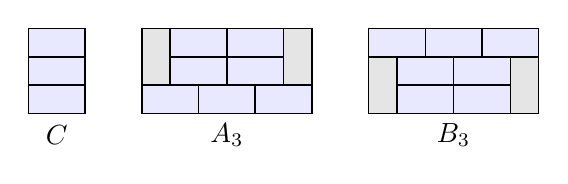
\begin{tikzpicture}[x=0.36cm,y=0.36cm,line width=0.55pt]
\begin{scope}
 \foreach \y in {0,1,2}{\draw[fill=blue!9] (0,\y) rectangle ++(2,1);}
 \node at (1,-0.75) {$C$};
\end{scope}
\begin{scope}[shift={(4,0)}]
 \draw[fill=gray!20] (0,1) rectangle (1,3);
 \draw[fill=gray!20] (5,1) rectangle (6,3);
 \foreach \x in {0,2,4}{\draw[fill=blue!9] (\x,0) rectangle ++(2,1);}
 \foreach \y in {1,2}{\foreach \x in {1,3}{\draw[fill=blue!9] (\x,\y) rectangle ++(2,1);}}
 \node at (3,-0.75) {$A_3$};
\end{scope}
\begin{scope}[shift={(12,0)}]
 \draw[fill=gray!20] (0,0) rectangle (1,2);
 \draw[fill=gray!20] (5,0) rectangle (6,2);
 \foreach \x in {0,2,4}{\draw[fill=blue!9] (\x,2) rectangle ++(2,1);}
 \foreach \y in {0,1}{\foreach \x in {1,3}{\draw[fill=blue!9] (\x,\y) rectangle ++(2,1);}}
 \node at (3,-0.75) {$B_3$};
\end{scope}
\end{tikzpicture}

\caption{Representative blocks $C,A_3,B_3$. Rectangle boundaries
are domino boundaries. The diagram was drawn from the coordinate
definitions using AI-assisted TikZ code.}\label{fig:blocks}
\end{figure}

\begin{lemma}\label{lem:word}
Every three-row tiling has a unique decomposition into a word
over $\mathcal B=\{C\}\cup\{A_k,B_k:k\ge1\}$.
Let $\sigma$ fix $C$ and interchange $A_k,B_k$.
Under this correspondence,
\begin{equation}\label{eq:word-action}
 h(W)=\sigma(W),\qquad v(W)=\rev(W),\qquad
 \rho(W)=\sigma(\rev(W)),
\end{equation}
where $\sigma$ is applied letterwise.
\end{lemma}
\begin{proof}
Cut a tiling at all its faults. The resulting pieces have no
internal faults and hence are precisely the blocks of Lemma
\ref{lem:blocks}. Every boundary in a block decomposition must
be a fault, and every fault must be used: omitting one would
leave a decomposable piece. This proves uniqueness.
Concatenation gives the inverse map, with the empty word
corresponding to the empty tiling.

Horizontal-axis reflection acts on individual blocks by $\sigma$.
Every block is invariant under vertical-axis reflection.
For $A_k$, the column reversal $c\mapsto2k+1-c$ interchanges
the endpoint vertical dominoes. It sends each bottom-row pair
$(2j-1,2j)$ to another such pair, with index $k+1-j$,
and each upper-row pair $(2j,2j+1)$ to another, with index $k-j$.
The block $C$ is fixed domino by domino. Since the two
reflections commute and $B_k=h(A_k)$, every $B_k$ is also
invariant under vertical-axis reflection.

Both reflections preserve the set of faults. Horizontal-axis
reflection preserves block order, whereas vertical-axis
reflection reverses it. Uniqueness of the decomposition now
gives \eqref{eq:word-action}, including when block widths differ.
\end{proof}

\subsection{Fixed words}
Assign weight $x$ to $C$ and $x^k$ to $A_k,B_k$.
The exponent records half the width.
The block generating function is
\begin{equation}\label{eq:F}
 F(x)=x+2\sum_{k\ge1}x^k=\frac{3x-x^2}{1-x}.
\end{equation}
Since $F(0)=0$, only finitely many words contribute to any
given coefficient.

\begin{proposition}\label{prop:fixed-gf}
The four fixed-point generating functions are
\begin{align}
D(x)&=\frac{1}{1-F(x)}=\frac{1-x}{1-4x+x^2},
&H(x)&=\frac{1}{1-x},\label{eq:DH}\\
V(x)&=(1+F(x))D(x^2)
 =\frac{1+3x+x^2-x^3}{1-4x^2+x^4},\label{eq:V}\\
R(x)&=(1+x)D(x^2)
 =\frac{1+x-x^2-x^3}{1-4x^2+x^4}.\label{eq:R}
\end{align}
\end{proposition}
\begin{proof}
An arbitrary word contributes to
$D=\sum_{\ell\ge0}F^\ell$.
A word fixed by $h$ must consist entirely of letters fixed by
$\sigma$. The only such letter is $C$, giving $H$.

A word fixed by $v$ is a palindrome. It has a unique expression
$U\rev(U)$ or $Ub\rev(U)$, where $b$ is any block.
The two copies of $U$ contribute $D(x^2)$, and the possible
central block contributes $1+F(x)$.

A word fixed by $\rho$ has a unique expression
$U\sigma(\rev(U))$, or $Ub\sigma(\rev(U))$ with $\sigma(b)=b$.
In the latter case $b=C$, so the central contribution is $1+x$.
In both constructions the two cases are disjoint and the
decomposition is reversible. A central block may cross the
geometric midline; that line is not required to be a fault.
\end{proof}

\begin{proof}[First proof of Theorem \ref{thm:main}]
Burnside's formula and Proposition \ref{prop:fixed-gf} give
\begin{equation}\label{eq:average-rational}
 A(x)=\frac14\left[
 \frac{1-x}{1-4x+x^2}+\frac1{1-x}
 +\frac{2(1+2x-x^3)}{1-4x^2+x^4}\right].
\end{equation}
Put $P_3=1-4x+x^2$ and $Q_3=1-4x^2+x^4$.
On taking the common denominator $(1-x)P_3Q_3$, its numerator is
\begin{align*}
 &\frac{(1-x)^2Q_3+P_3Q_3+
 2(1+2x-x^3)(1-x)P_3}{4}\\
 &\hspace{35mm}=1-3x-4x^2+10x^3-4x^5+x^6.
\end{align*}
This proves \eqref{eq:main}. The denominator expands to
\[
 1-5x+x^2+19x^3-19x^4-x^5+5x^6-x^7.
\]
The numerator has degree six, so comparison of coefficients
of $x^n$ for $n\ge7$ gives \eqref{eq:recurrence}.
The coefficients of degrees zero through six give the initial
values in the theorem.
\end{proof}

\begin{remark}
In \cite[equation (26)]{mathar2013}, the variable $z$ marks the
full width, so the appropriate comparison is
$\overline T(z,3)=A(z^2)$.
After substitution into \eqref{eq:average-rational}, the
horizontal-reflection contribution $H(z^2)/4$ can be written as
\[
 \frac18\left(\frac1{1+z}+\frac1{1-z}\right)
 =\frac1{4(1-z^2)},
\]
Rearranging the other contributions gives the cited expression.
In the three-row formulas of
\cite[equations (4)--(6)]{mathar2014}, $z$ instead marks the
number of dominoes; the corresponding substitution is $z^3=x$.
\end{remark}
